\paragraph{Цель работы:} Промоделировать работу промышленного робота RV-2AJ.

\subsection*{Выполнение}

\begin{enumerate}
	\item Создание нового проекта с роботом RV-2AJ.
	\item Добавление примитивов (куба и цилиндра), редактирование примитивов, обнаружение коллизий.
	\item Настройка точек захвата.
	\item Сохранение точек схвата ПР: начальная точка, подведение схвата к заготовке, подведение схвата к конечной точке.
	\item Написание программы перемещения роботом ``синего куба'' на ``желтый цилиндр'', а потом возврата заготовки обратно.
	\item Запуск программы.
\end{enumerate}

Скриншоты выполнения лабораторной работы прилагаются в Приложении А.

\subsection*{Листинг программы}

\begin{verbatim}
20 MVS P1
30 HOPEN 1
40 MVS P2,-40
50 HCLOSE 1
60 DLY 0.2
70 MVS P3,-40
80 HOPEN 1
90 DLY 0.2
100 MVS P1
110 END
\end{verbatim}

\subsection*{Выводы}

Программный пакет ``COSIMIR Professional'' служит для симуляции промышленных роботов и моделирования производственных участков, состоящих из робота и деталей, с которыми необходимо провести определенные операции. В этой лабораторной работе мы промоделировали перемещение заготовки кубической формы из начальной точки в точку транспортировки при помощи схвата промышленного робота RV-2AJ, написали и запустили программу на языке MELFA-BASIC IV/V, разобрались с возникнувшими вопросами и трудностями.

\clearpage

\subsection*{Приложение А}

\begin{figure}[ht]
\centering
	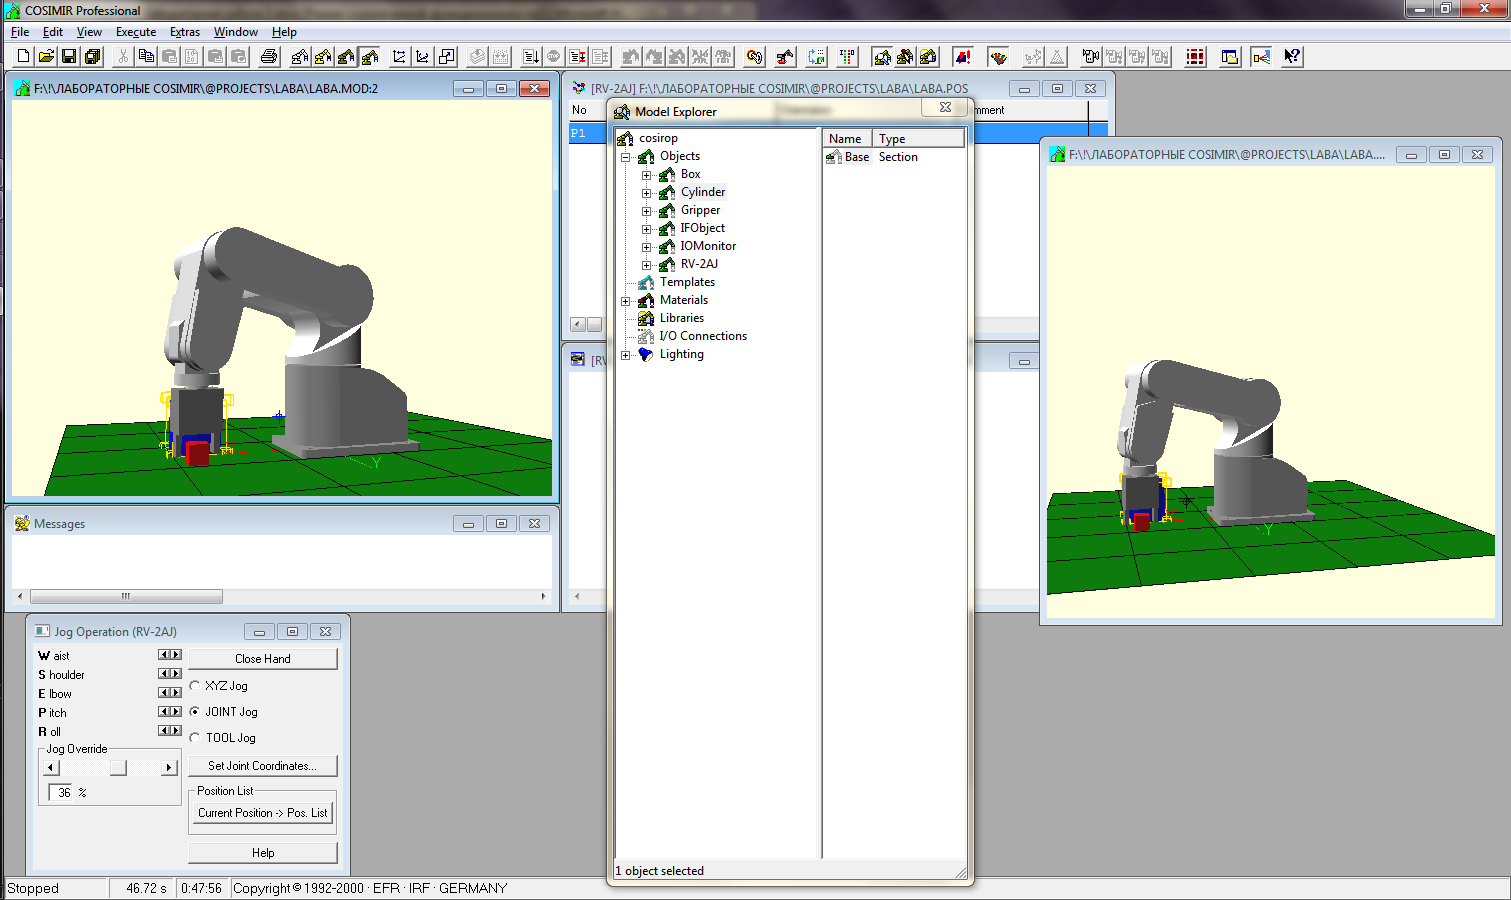
\includegraphics[scale=0.35]{1.png}
	\caption{Результат выполнения работы}
\end{figure}

\begin{figure}[ht]
\centering
	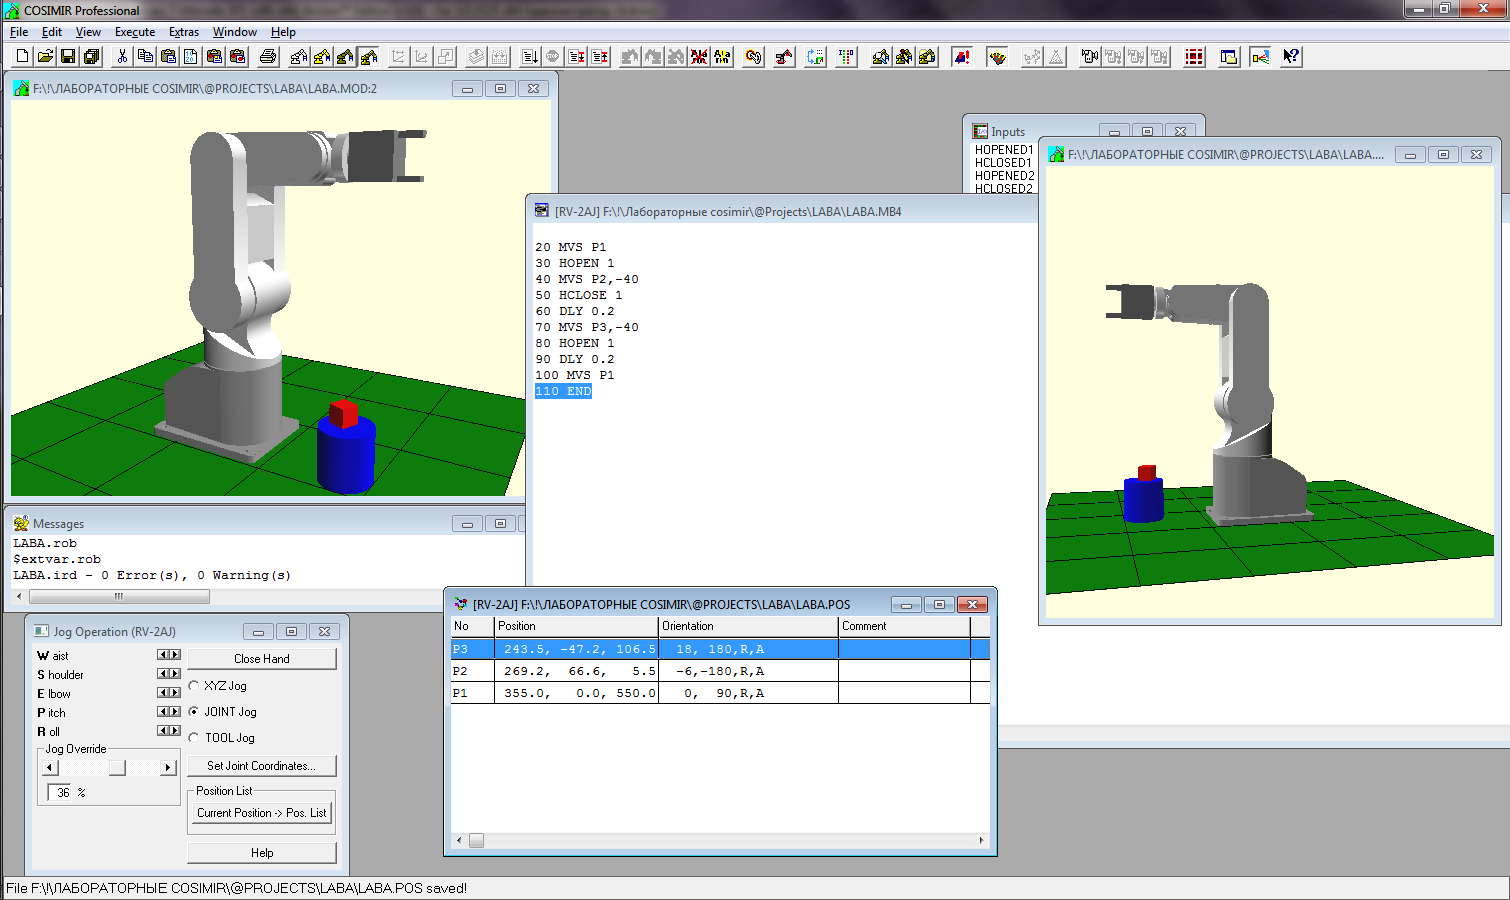
\includegraphics[scale=0.35]{2.png}
	\caption{Результат выполнения работы}
\end{figure}

\begin{figure}[ht]
\centering
	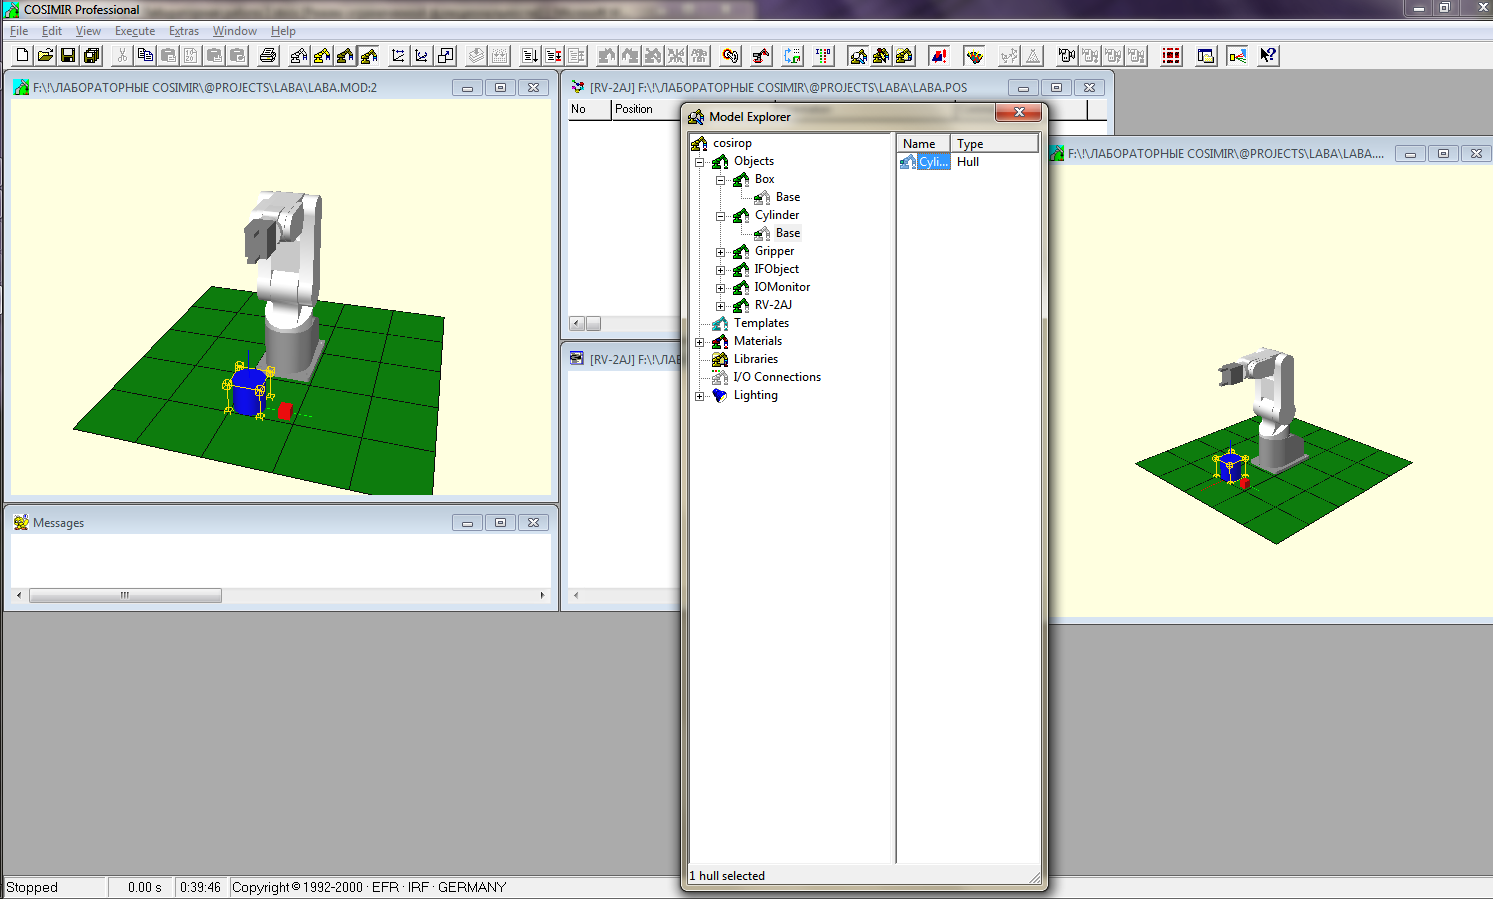
\includegraphics[scale=0.4]{3.png}
	\caption{Результат выполнения работы}
\end{figure}

\begin{figure}[ht]
\centering
	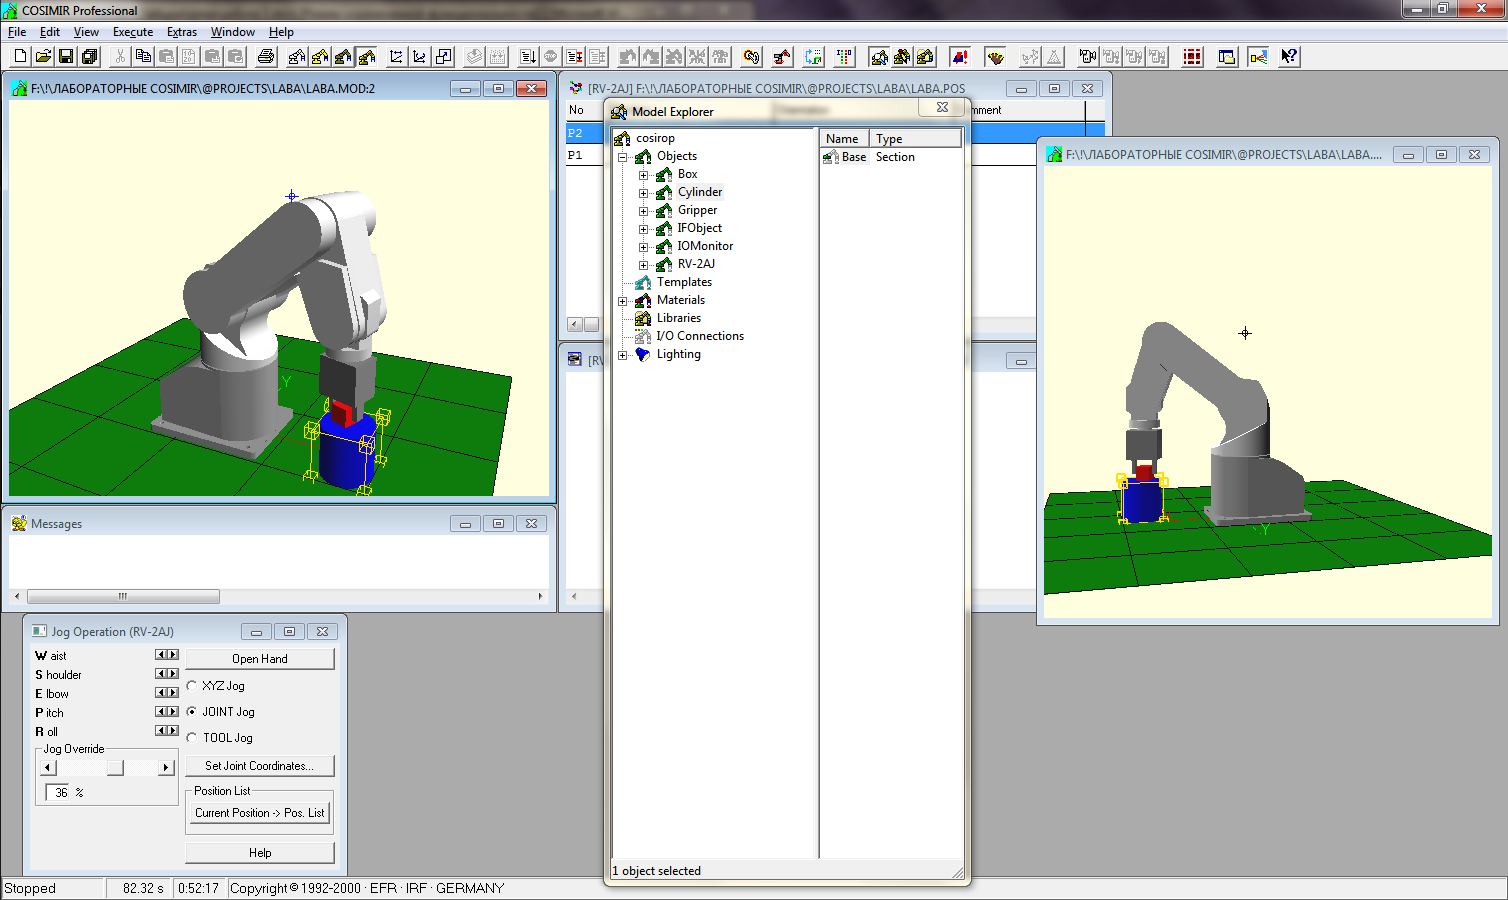
\includegraphics[scale=0.4]{4.png}
	\caption{Результат выполнения работы}
\end{figure}

\clearpage